\RequirePackage[hyphens]{url}
\documentclass[11pt,titlepage,dvipsnames,table,xcdraw]{article}
\usepackage{strath-dissertation}
\usepackage{setspace}

\usepackage{babel}
\usepackage{lipsum} % For demonstration only.
\usepackage{graphicx}
\usepackage{subfigure}
\usepackage{caption}
\usepackage{subcaption}
\usepackage{enumitem}
\usepackage{multicol}


%--------------------------------
% Degree settings
%--------------------------------
\newcommand{\degreename}{Bachelor of Science}
\newcommand{\coursename}{CS408: Individual Project}
\newcommand{\deptname}{Computer and Information Sciences}

\begin{document}

%--------------------------------
% Title page.
%--------------------------------
\begin{titlepage}
\vspace*{5mm}
\titletext{Implementing the Chinese Wall Security Model in Security Enhanced Linux}
\vspace{10mm}
\authortext{Calum Cardownie}
\vspace{15mm}
\centering{\Large{\textbf{Progress Report}}}
\vspace{40mm}
\centredcrest
\vspace{5mm}
\depttext{\deptname}
\vspace{5mm}
\datetext{November, 2025}
\end{titlepage}

%--------------------------------
% Front matter numbering.
%--------------------------------
\pagenumbering{roman}
\setcounter{page}{2}

%--------------------------------
% Setting counter depth.
%--------------------------------
\setcounter{secnumdepth}{3}
\setcounter{tocdepth}{2}

%--------------------------------
% The front matter.
%--------------------------------
\setstretch{1.2} % 1.5 line spacing. 


%--------------------------------
% Tables of contents.
%--------------------------------
\setstretch{1.0} % 1.0 line spacing.  
\clearpage
\tableofcontents
%\listoffigures   % Uncomment for a list of figures.
%\listoftables    % Uncomment for a list of tables.
\clearpage

%--------------------------------
% The body of the document.
%--------------------------------
\pagenumbering{arabic} % Page numbering for rest of document.
\setstretch{1.5} % 1.5 line spacing. 


\section{Aims and Objectives}

\subsection{Aims}
The aim of this project is to understand, define and implement the Chinese Wall security model in Security Enhanced Linux (SELinux).
As a Chinese Wall in SELinux has never been documented before, this project will document the creation and challenges of implementing the dynamic model in the generally static SELinux environment.
As such, the objectives include:

\subsection{Objectives}
\begin{enumerate}[label=1.\arabic*]
  \item Creating a suitable environment for SELinux
  \item Understanding the principles of
    \begin{enumerate}[label=1.2.\arabic*]
    \item The Chinese Wall Security model
    \item SELinux and its security capabilities
  \end{enumerate}
  \item Defining the Chinese Wall model and its actions in response to \verb_CoI_ breaches
  \item Creating a static implementation of the policy in SELinux
  \item Creating a daemon that is capable of monitoring subjects and the objects they access
  \item Adapting the daemon to dynamically update labels to achieve the complete Chinese Wall Security model
  \item Analyze the difficulties that arose from development and conclude why research in this area has been lacklustre
\end{enumerate}

\subsection{Opening Notes}
As this implementation is new ground, it must also be considered that a Chinese Wall model in SELinux may be exceptionally challenging. The analysis stage will examine the results regardless of if the Chinese Wall is achieved, but a working implementation still remains
a priority of this project. This may mean that this paper's future work might delve into adjacent areas, potentially exploring the
viability of a Chinese Wall model in related systems, if the Wall cannot be implemented.

\clearpage

\section{Summary of Related Work}

\subsection{Chinese Wall Model Origin}
The Chinese Wall security model - or Brewer and Nash model \cite{brewer_chinese_1989} - is a security model that prevents information from conflicts of interest (\verb_CoI_) groups being spread. 
As opposed to the Bell LaPadula (BLP) model, which enforces "no read up, no write down" \cite{bell_secure_1973}, the Chinese Wall model allows for information flow freely until a subject (e.g. a user or process) attempts to read
from a \verb_CoI_ object (piece of information). Upon this access, the system dynamically revokes their write permissions to other objects in the \verb_CoI_ group,
creating a "wall" in-between them. Consider the following scenario: 

A data server stores information on Banks A and B, and Oil Company A and B. These are in \verb_CoI_ groups with their respective counterpart. If a user approaches the dataset, they are initially able to access
any object. As far as the system knows, this user is free as they have no prior knowledge of either companies. Suppose the user has read from Bank A, the situation develops - the user now possesses
information that, deemed by the Chinese Wall, should not be allowed to reach Bank B, as they are conflicting with Bank A. This is where the wall revokes the write access from the user in regard to Bank B.
Now information \textit{cannot} flow from Bank A to B. 

\begin{itemize}
  \item \textbf{BN Read Rule}: Subject \verb_S_ can read object \verb_O_ only if \verb_O_ is in the same Company Dataset \verb_(CD)_ as an object already read by \verb_S_, or if \verb_O's_ \verb_(CD)_ is in a 
    different Conflict of Interest \verb_(CoI)_ group from all \verb_CDs_ of objects already read by \verb_S_.
  \item \textbf{BN Write Rule}: Subject \verb_S_ can write to an object \verb_O_ only if \verb_S_ can read \verb_O_ \textbf{and} all objects \verb_O'_ read by \verb_S_ are in the same \verb_CD_ as \verb_O_.

\end{itemize}

The Brewer Nash model provides a mathematical format that is based on the larger Chinese Wall policy, a pillar of compliance in the financial sector.
Chinese Walls are a common practice that should theoretically and practically prevent misuse of probable information leakage in banks \cite{herzel_chinese_1978} and other financial management firms.
After the Brewer Nash model was communicated, another paper was published once again by Brewer and Nash, but also TY Lin, who presented them with potential improvements on their model \cite{lin_chinese_1989},
leading to the Aggressive Chinese Wall. This idea, trying to disprove the assumption that the conflict of interest is an equivalent relation, has been accepted into the mainstream since it was
proposed. This is the type of implementation the 1997 UNIX proof believed in \cite{foley_building_1997}, illustrating the possibility of its creation in UNIX. Such proofs in UNIX lead it to be assumed to
theoretically be possible in Linux and SELinux. This proof indicates there is research, but there is a lack of documented attempts to specifically implement it into the UNIX or adjacent kernel.

\subsection{Security Enhanced Linux}
Security Enhanced Linux implements a Mandatory Access Control (MAC) system, providing a policy-driven security layer extended beyond the classic
Discretionary Access Control (DAC) system that UNIX based systems use. DAC is defined such that objects and their privileges are managed by whoever made them, and the root user can access and 
control anything. DAC in UNIX leverages the \verb_chmod_ (change mode) command, allowing read, write and execute access of objects to be edited for the 3 main groups subjects can belong to. While DAC brings about great
flexibility, the models' reliance on ownership often leads to uncontrolled privilege propagation. It is known to be difficult to measure the security of the DAC model, and in some cases it is undecidable \cite{fan_mandatory_2009}. 
MAC is the other model that shares the spotlight with DAC in system security. It utilises, labels, attached to both subjects and objects. Installed policies into the security server govern what labels can interact.
Labels are devised in the form \verb|user_u:role_r:type_t:c0|
For instance, a base policy may be that an object of type \verb|httpd_t| can only be operated on by a subject of 
type \verb|httpd_t| and not \verb|sshd_t|. This provides strong mitigation against
broken access control damages, as subjects can only access objects that they should and are unable to change the policy controls. For this reason SELinux is adopted by many distributions of Linux, including Red Hat,
Fedora, CentOS and even mobile operating system giant Android. SELinux is based off of the Flux Advanced Security Kernel (FLASK) security architecture for flexible
nondiscretionary access controls, where the architecture is split into policy enforcement and policy decision-making. 
SELinux's origin can be attributed to the National Security Agency's Trusted UNIX (TRUSIX) Working Group, working together to publish a Rainbow Book (A series of Computer Security standards and guidelines
by the United States Government), and created a second (unpublished) book that included a formal SELinux model and associated evaluation evidence prototype. SELinux was a demonstration that mandatory access
control was viable and could be added to the Linux kernel, and so it was merged into the mainline kernel in the 2.6 series of the kernel. Linux was able to adopt this because of its derivation from UNIX, Linux
being an open source alternative to the UNIX that was locked down by AT&T. Linus Torvalds combined his Linux kernel with the GNU system tools to create GNU/Linux, leading to what we now know as Linux. This open-source
philosophy and flexibility were key factors enabling SELinux's integration into the mainline kernel in the 2.6 series.

\subsection{Chinese Wall Model in System Security}
Cloud computing is an avenue that has had a successful Chinese Wall model implementation \cite{tsai_practical_2011}. 
In this case,
there are many Virtual Machines (VMs) running on one system, with the virtual machine monitor, or "hypervisor" acting as the delegating force of the computers' hardware. Each virtual machine 
is a separate operating system, commonly being completely independent of the other VMs on a machine. Inter-VM attacks can happen if a VM on the system is breached, and can lead to one infected
VM spreading to the whole system. This is where the Chinese Wall was 
created, to eliminate the possibility of inter-VM attacks from competitors. The security model was implemented on the Kernel-base Virtual Machine (KVM) level.
Once a VM in a \verb_CoI_ group is running on a physical host, the Wall prevents other VMs belonging to the same \verb_CoI_ group from being scheduled on the same machine. This effectively eliminates the risk of
inter-VM attacks in these systems.

Beyond virtualized environments,
the Chinese Wall model has also successfully been implemented in workflow management systems. Workflow Management Systems (WfMS) are intrinsically network-based applications, potentially hosting multiple conflicting
sources of information. As such, a secure WfMS must implement security features, specifically targeting information confidentiality as a main point of effort. The Chinese Wall security model can be leveraged
to prevent conflict of interest leakage. A Chinese Wall was implemented using role-based access control (RBAC) to enforce, and Java to handle the Chinese Wall logic \cite{hsiao_implementing_2010}. The paper
mentions that RBAC is unable to implement general cases of the Chinese Wall, as it has issues implementing the BN read rule in dynamic contexts. 


\clearpage

\section{Project Specification}

\subsection{Functional and Non-Functional Requirements}
Functional Requirements: 
\begin{itemize}
  \item \verb_cwalld_ must run as a daemon in the user-space of the computer until terminated
  \item \verb_cwalld_ must monitor read and write actions on all subjects on the system
  \item \verb_cwalld_ must identify \verb_CoI_ triggers to act upon
  \item \verb_cwalld_ must create a policy module that will prevent the \verb_CoI_ from being breached
  \item \verb_cwalld_ must install the policy on the machine
  \item \verb_cwalld_ will write to a log file documenting policies it installs
\end{itemize}

Non-Functional Requirements:
\begin{itemize}
  \item \verb_cwalld_ will only be controllable by the admin
  \item \verb_cwalld_ will handle memory in a thread-safe and careful manner such to avoid concurrency issues and memory leaks
  \item \verb_cwalld_ must not significantly impact performance of the system
\end{itemize}

\subsection{Technology Selection: C Programming Language}

The Chinese Wall security daemon will be implemented in \verb_C_, elected for its suitability for kernel and system-level programming. The main reasons for this choice are documented below

\begin{itemize}
  \item \textbf{System Program Status}: \verb_C_ has been the \textit{de-facto} standard language for operating systems programming since its origin in the 1970s, with major kernels including Linux, Windows NT and freeBSD
    being predominantly written in \verb_C_.

  \item \textbf{Low-level Precision}: \verb_C_ is a language that allows the developer incredible freedom, including the potential to manipulate memory directly, and interact with core parts of the system. The daemon requires
    direct interaction with system calls and process management, which \verb_C_ provides natively.

  \item \textbf{Performance}: \verb_C_ is a compiled language with minute overhead, ensuring that the daemon introduces minimal latency to the system.

  \item \textbf{Familiarity}: I have prior experience with \verb_C_, developing several low level projects with it, courtesy of CS210.
\end{itemize}

The use of \verb_C_ introduces some challenges however, listed below

\begin{itemize}
  \item \textbf{Memory Management}: Given \verb_C_ grants the developer power to manipulate memory, it must be managed with disciplined design practices. If memory is not managed perfectly it can lead to
    memory leaks and buffer overflows, that will build up and completely eliminate the daemon's viability.

  \item \textbf{Concurrency}: System daemon tasks inherently involve concurrency, as such practices such as mutex locks and semaphores must be considered to prevent race conditions, and the daemon must follow
    thread-safe design patterns.
\end{itemize}

\subsection{Other Language Avenues}

Other languages that were considered include:

\begin{itemize}
  \item \textbf{Rust}: \verb_Rust_ is hailed for its type safety and security, while also compiling to near C-level speed, making it a great choice for daemon development, however, the steep learning curve makes it 
    a difficult choice.
  \item \textbf{Go}: \verb_Go_ is a modern, slightly higher level alternative to \verb_C_, with excellent concurrent integration with its Goroutines, but the garbage collection introduces latency
    and an indirect method of interaction with SELinux libraries leave it in the shadow of \verb_C_.
  \item \textbf{Python}: While recent developments with \verb_Python 3.14_ have removed the global interpreter lock that prevented true multithreading, it remains an interpreted language that cannot match the 
    speed and minimal overhead of compiled languages such as \verb_C_.
\end{itemize}



\clearpage
\section{Project Plan including summary of progress}
The project has 3 main phases. 
\begin{itemize}
  \item \textbf{Phase 1}. Developing a static Chinese Wall in SELinux
  \item \textbf{Phase 2}. Achieving a dynamic Chinese Wall security model
  \item \textbf{Phase 3}. Analyzing the journey of the project and concluding why it has been void of attention
\end{itemize}

The setup for the first phase involves setting up an environment that can run SELinux. I have chosen Red Hat as the Linux distribution for this end. Red Hat Enterprise Linux (RHEL) is a popular SELinux distribution 
that other distributions like Fedora and CentOS are forks and inspired by respectively. The plan outlines using a combination of Kernal-based Virtual Machine (KVM) and Quick Emulator (QEMU) to run
the VM. Virt manager, created by the same company as Red Hat, IBM, was chosen to act as an interface to run and interact with the VM. The details of the VM can be found
in figure: \ref{redhat} in the appendix.

\subsection{Phase 1: Developing a static Chinese wall in SELinux}
The first phase is based on researching and understanding the capabilities of SELinux, and the completion of a static Chinese Wall. The plan for this phase involves scoping out the capabilities of SELinux's security
system. So far, a static implementation of a Chinese Wall has been the priority. This involves an object, able to be written and read by subject A, but not subject B, whilst the subjects having the same access 
everywhere else in the system. This must be implemented with SELinux security
labels for properly enforced security. In pursuit of the static wall and pushing the limits of SELinux, I have learnt many things about SELinux systems, including:
\begin{itemize}
  \item Familiarisation with SELinux libraries (SETroubleshoot, Policycoreutils, SETools-console)
  \item Identification and modification of SELinux labels and object access
  \item Creating and confining a simple daemon within an SELinux context 
  \item Creating and installing SELinux type enforcement files
\end{itemize}

At this point, a base static wall has been completed. I began by attempting to enforce the wall on a user basis, preventing a real Linux user from accessing objects they were in conflict with.
It is very difficult to adapt the type of specifically the user, using a process rather than a standard system running subject. As such, the Chinese Wall may only be able to enforce
its protection on a process level and not a system user level.

\subsection{Phase 2: Achieving a dynamic Chinese Wall security model}
The plan for the second phase primarily involves creation of the Chinese Wall daemon, written in \verb_C_. This daemon will survey the system and modify security modules, designating the denial to the security server.
This will be the longest phase, including daemon development, along with testing. Phase 2 will also potentially venture into Kernel level engineering, as a Chinese Wall will require atomic operations to deny subjects
based on their history, and installing policy modules is a system-wide operation that will not be able to done freely by a daemon.

\subsection{Phase 3: Analysing the journey to making the Chinese Wall model in SELinux}
The final phase is simply analysing challenges that arose from creation of the wall. The main challenge so far has been a lack of documentation. While the Red Hat docs are well-written and detailed, they only describe
operations that a standard system admin would need, rather than anything more complex like custom policy modules. As such, finding accurate documentation is a challenge for this project, as SELinux has its own policy
module language (.te) with its own syntax and logic system.

A Gantt chart was constructed to depict the project timeline:

\begin{figure}[h]
  \centering
  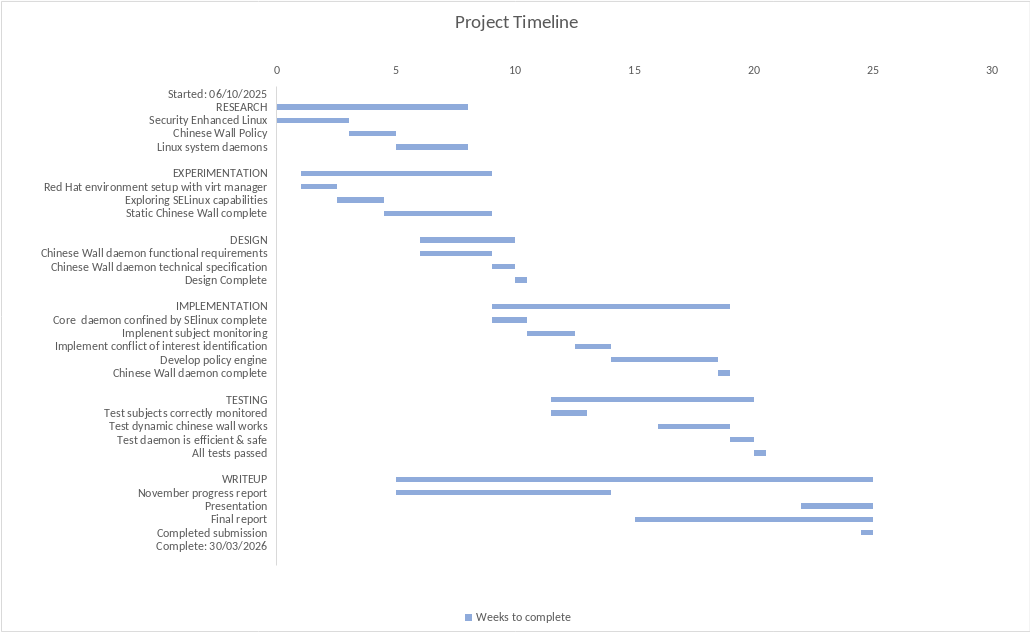
\includegraphics[width=0.95\linewidth]{figs/ganttchart.png}
  \caption{Project Gantt chart}
\end{figure}

\clearpage

\section{Approach to Development}

\subsection{Methodology}

As mentioned earlier, the project has 3 phases. Each phase will refer to a different style of development methodology.
The first phase is based on researching and understanding the capabilities of SELinux, and the completion of a static Chinese Wall. This phase is agile, as the needs of the phase will constantly be revisited 
and analysed. It will allow me to alter the functional and non-functional requirements of the daemon as I scope the SELinux environment out. 
The second phase will oversee the development process of the Chinese Wall daemon, introduced to the world as \verb_cwalld_. This phase will follow the waterfall principle. By this phase, the daemon will have 
a set of defined requirements, and all focus will be on developing the daemon to meet those ends. Regardless of phase 2's success, there will be enough time to approach phase 3. Phase 3 will delve into the reasoning behind the lack 
of Chinese Wall development in SELinux.

\subsection{Design}

The design of the Chinese Wall security policy is such that once a subject reads from an object that is related to a conflict of interest group, their write access to other objects within that conflict of interest
is revoked. This prevents information from one object to reach a competitor. 

SELinux is designed such that only subjects can only access objects if they have matching labels. In standard SELinux, these labels are all static and are only changed by the user under unique circumstances.
Allowing dynamic policies would involve having type enforcement (.te) files edited and installed live based on the labels of the subjects. This is where the Chinese Wall daemon is required.

\subsection{Implementation and Technology ideas}

The base language C comes completely fresh. As such, there will be usages of common C libraries, ranging from the standard library, daemon infrastructure, SELinux core, process monitoring
and system operations. The project will likely also involve kernel programming, which is notoriously difficult. This will be evaluated once that stage is reached.

\subsection{Testing and Evaluation plans}

Testing depends on the amount of time that remains once the daemon is complete, as it being operational will be a big bottleneck for the project. Once ready the daemon will be tested in efficiency, robustness
security. The daemon's resource usage will be measured and compared to other system daemons. Measuring robustness and security, the daemon will be tested to operate on a huge amount of subjects and objects at once,
and it will be noted if it was able to efficiently execute its operations without issue. The report will be evaluated based on the completion of the daemon, and it's ability to enforce the Chinese Wall security
policy.


\clearpage


\clearpage

%--------------------------------
% Bibliography
%--------------------------------
\clearpage
\setstretch{1.0}  % 1.0 line spacing. 
\bibliographystyle{abbrv}
\bibliography{bibliography}
% add references to the file called bibliography.bib
\clearpage

\appendix
\section{Red Hat System Specs}

\begin{figure}[h]
  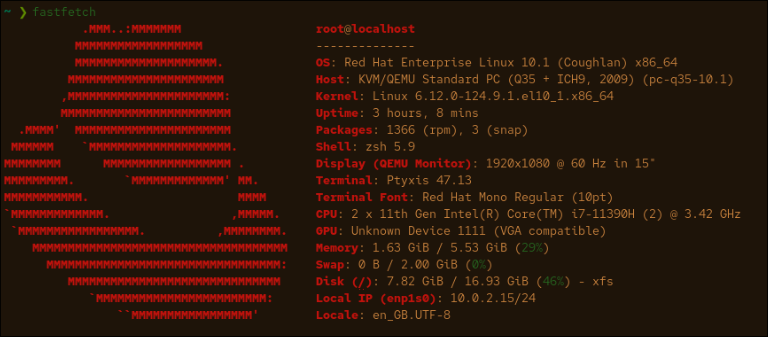
\includegraphics[width=1\linewidth]{figs/specs.png}
  \caption{Red Hat system specs}\label{redhat}
\end{figure}

\end{document}
